\chapter{システム構成およびデータ収集}

% =====================
% システム全体アーキテクチャ
% =====================
\section{システム全体アーキテクチャ}
本システムは,大別して3層からなるアーキテクチャで構成される（図\ref{fig:system}）.

\begin{figure}[htbp]
    \centering
    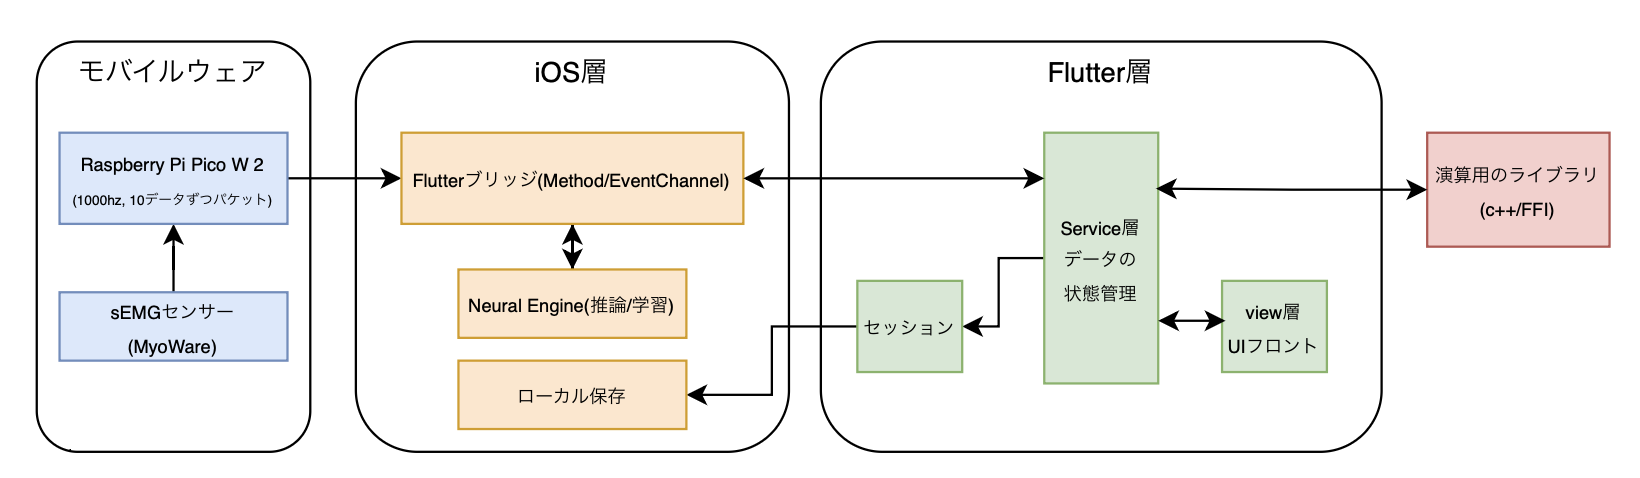
\includegraphics[width=\linewidth]{src/system.png}
    \caption{システム全体アーキテクチャ}
    \label{fig:system}
\end{figure}
    
\subsection{全体構成}
\begin{enumerate}
\item \textbf{モバイルウェア層（ペリフェラルデバイス）}\\
Raspberry Pi Pico 2 W とMyoWareセンサーで構成される.1kHzサンプリングでADC変換したsEMG信号を,10サンプルずつパケットしてNotifyする.

\item \textbf{iOS層（ネイティブ実行環境）}\\
FlutterブリッジがMethod Channel / Event Channelを介してFlutter層と通信し,Neural Engine（Core ML）を用いた推論・on-device学習,ローカルストレージへのセッション永続化を担当する.

\item \textbf{Flutter層（アプリケーション層）}\\
BLE通信,データバッファリング,セッション管理を行うService層,UIを提供するView層,高速演算を担うC++/FFIライブラリ（特徴抽出）から構成される.
\end{enumerate}

\pagebreak

\subsection{データフロー}
データは以下の流れで処理される：

\begin{enumerate}
\item Pico 2 Wが1kHzでsEMG信号をサンプリング
\item BLE経由で10サンプル/パケット（約100Hz）でFlutter層へ送信
\item Flutter Service層がバッファリング・セッション管理
\item C++ライブラリが150msウィンドウ（50msホップ）で特徴抽出（10次元特徴量）
\item iOS層のCore MLが特徴量からジェスチャ分類推論
\item View層がリアルタイム表示・データ記録
\end{enumerate}

\pagebreak


% =====================
% ハードウェア構成
% ====================
\section{ハードウェア構成}
本システムで使用するハードウェアコンポーネントの仕様を以下に示す.
Raspberry Pi Pico 2 W をマイコンとして利用し電源とアナログセンサーの値取得を行い,BLE経由でモバイル端末へ送信する.

\subsection{ハードウェアの選定}
\begin{table}[htbp]
\centering
\caption{ハードウェア構成一覧}
\label{tab:hardware}
\begin{tabular}{lll}
\hline
\textbf{コンポーネント} & \textbf{型番/仕様} & \textbf{用途} \\ \hline
マイコン & Raspberry Pi Pico 2 W & 信号サンプリング・BLE通信 \\
sEMGセンサー & MyoWare 2.0 筋電位センサー & 表面筋電位計測 \\
開発環境 & MicroPython & ファームウェア実装 \\ \hline
\end{tabular}
\end{table}

\subsection{ファームウェア（Raspberry Pi Pico 2 W）}
MicroPythonベースのBLE Peripheral実装により,以下の機能を提供する：

\begin{itemize}
\item \textbf{サンプリング}：内蔵ADC4を用いた1kHz連続サンプリング
\item \textbf{パケット}  ：シーケンス番号（2バイト）+ 10サンプル（各4バイトfloat）の42バイト
\item \textbf{送信レート}：100Hz（10パケット周期）でNotify配信
\end{itemize}

\pagebreak

% =====================
% ソフトウェア構成
% =====================
\section{ソフトウェア構成}
Flutterにおけるメインアプリケーションのソフトウェア構成はクリーンアーキテクチャを採用し,それぞれのパイプラインや演算処理をServiceとして定義したのちインスタンスをRiverpodで状態管理して各UIで参照する.
（図\ref{fig:flutter-arch}）

\begin{figure}[htbp]
    \centering
    \begin{tikzpicture}[
      font=\small,
      node distance=8mm and 15mm,
      box/.style={draw, rounded corners, align=center, minimum width=30mm, minimum height=9mm},
      arrow/.style={-Latex, thick}
    ]
  
      % Widgets層
      \node[box, fill=blue!10] (widgets) {Widgets};
  
      % Riverpod Providers層
      \node[box, fill=green!10, below=of widgets] (providers) {Riverpod Providers};
  
      % Services層
      \node[box, fill=orange!10, below=of providers] (services) {Services};
  
      % 矢印（Providersがインスタンスを生成・注入）
      \draw[arrow] (providers) -- node[left]{\footnotesize インスタンス生成} (services);
      \draw[arrow] (providers) -- node[right]{\footnotesize 依存性注入} (widgets);
  
      % Services層の詳細（右側に配置）
      \node[align=left, font=\footnotesize, right=25mm of providers, anchor=west] (services-detail) {
        \textbf{Service群}\\
        - BleService: BLE通信処理\\
        - EmgMlService: Modelの読み込み,推論,学習\\
        - EmgWindowBuffer: センサデータのwindow buffer\\
        - EmgDatasetRecorder: データセットの記録\\
        - EmgFeatureExtractor: 特徴量の抽出
      };
  
    \end{tikzpicture}
    \caption{Flutter層のアーキテクチャ構成とRiverpodによる状態管理}
    \label{fig:flutter-arch}  
\end{figure}

\begin{figure}[htbp]
    \centering
    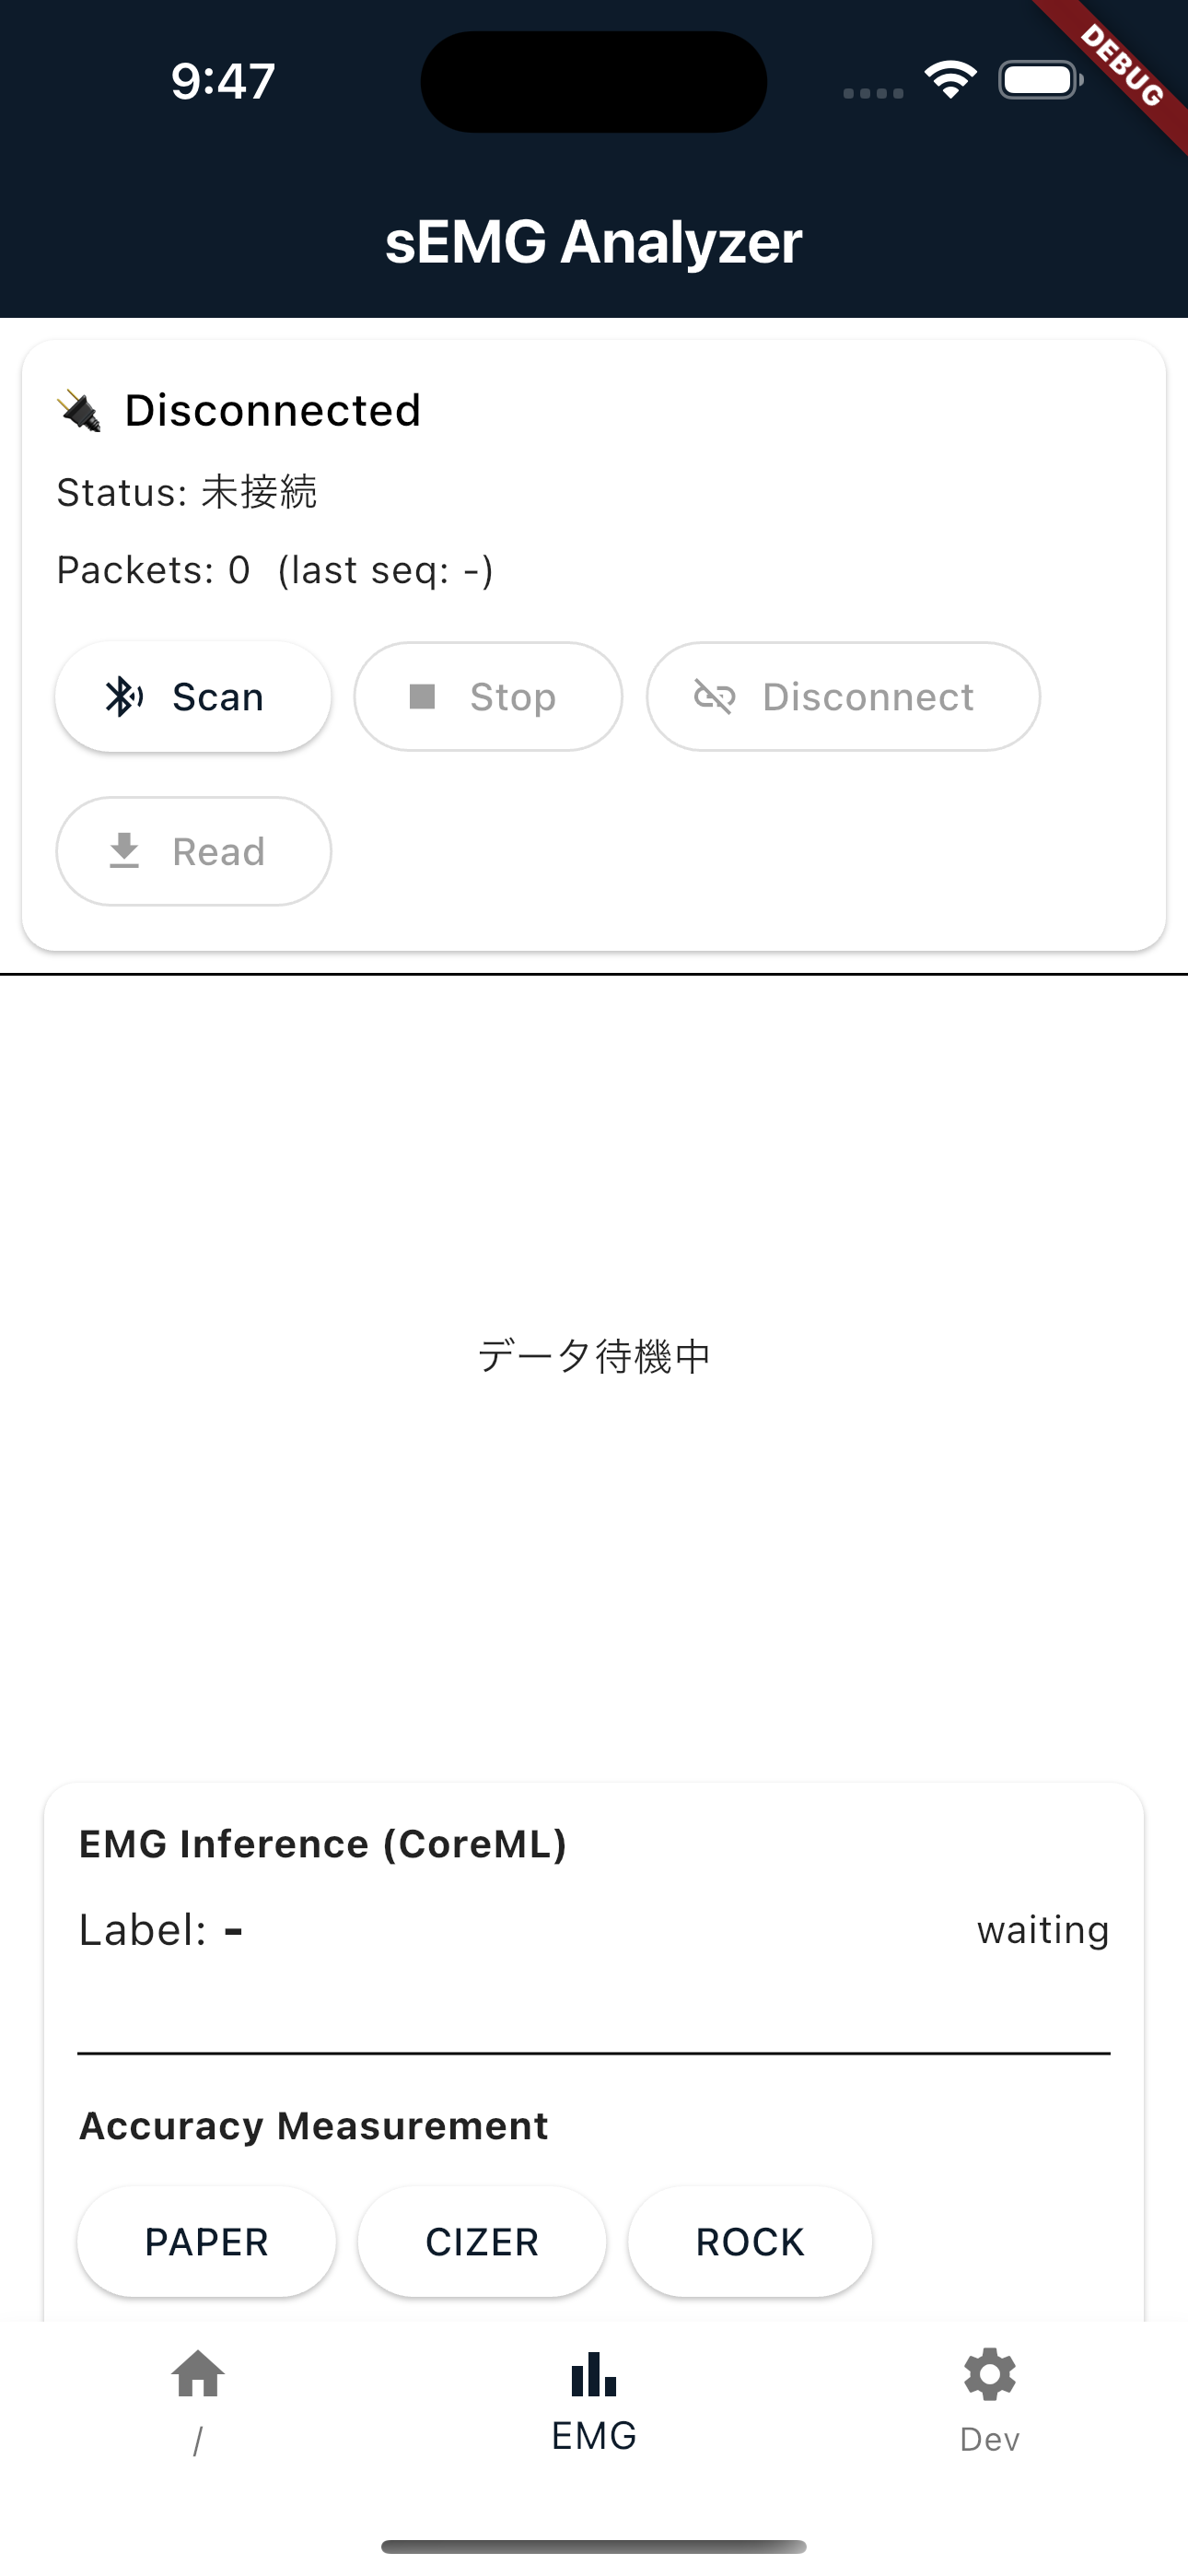
\includegraphics[width=0.3\linewidth]{src/idling_screen.png}
    \caption{アプリケーションのアイドリング状態画面}
    \label{fig:idling-screen}
\end{figure}

\subsection{実装したServiceクラス群}
本システムでは,データフロー上の各処理をServiceクラスとして分離し,
Riverpod Providersによる依存性注入により結合している.
以下に各Serviceの役割を示す.

\subsubsection{BleService（BLE通信）}
\label{subsubsec:ble-service}
Raspberry Pi Pico 2 WとのBLE通信を担当.
\texttt{flutter\_blue\_plus}によりBLE Central機能を実装し,
デバイス名でフィルタリング後,カスタムUUIDのキャラクタリスティックからNotify購読する.
42バイトパケット（シーケンス2B + 10サンプル40B）を\texttt{BleDataPacket}としてStreamで配信（図\ref{fig:ble-flow}参照）.

\begin{figure}[htbp]
    \centering
    \begin{tikzpicture}[
      font=\footnotesize,
      node distance=6mm,
      box/.style={draw, rounded corners, align=center, minimum width=22mm, minimum height=7mm},
      arrow/.style={-Latex, thick}
    ]
  
      \node[box, fill=blue!10] (scan) {スキャン};
      \node[box, fill=blue!10, right=of scan] (connect) {接続};
      \node[box, fill=green!10, right=of connect] (notify) {Notify};
      \node[box, fill=orange!10, right=of notify] (parse) {パース};
      \node[box, fill=red!10, right=of parse] (stream) {Stream};
  
      \draw[arrow] (scan) -- (connect);
      \draw[arrow] (connect) -- (notify);
      \draw[arrow] (notify) -- (parse);
      \draw[arrow] (parse) -- (stream);
  
      % パケット構造（下部）
      \node[below=12mm of notify, align=center, font=\footnotesize] (packet) {
        \textbf{パケット}\\
        {[}seq:2B{]} + {[}10samples:40B{]}
      };
  
    \end{tikzpicture}
    \caption{BLE通信フローとパケット構造}
    \label{fig:ble-flow}
\end{figure}

\subsubsection{EmgWindowBuffer（データバッファリング）}
\label{subsubsec:window-buffer}
連続サンプルを時系列バッファに蓄積し,150サンプル（150ms）のウィンドウを50サンプル（50ms）ホップで切り出す.
2/3オーバーラップで特徴量を抽出する.（図\ref{fig:window-buffer}参照）.

\begin{figure}[htbp]
    \centering
    \begin{tikzpicture}[
      font=\footnotesize,
      box/.style={draw, minimum width=3mm, minimum height=6mm, inner sep=0pt}
    ]
  
      % 連続データストリーム
      \foreach \i in {0,...,19} {
        \node[box, fill=gray!20] at (\i*0.3, 0) {};
      }
      \node[right] at (6, 0) {\footnotesize 連続データストリーム};
  
      % Window 1
      \draw[red, very thick] (0, 0.4) rectangle (1.35, -0.4);
      \node[red, above] at (0.675, 0.5) {Win1 (150)};
  
      % Window 2
      \draw[blue, very thick] (0.45, 0.3) rectangle (1.8, -0.3);
      \node[blue, above] at (1.125, 0.8) {Win2};
  
      % Window 3
      \draw[green!60!black, very thick] (0.9, 0.2) rectangle (2.25, -0.2);
      \node[green!60!black, above] at (1.575, 1.1) {Win3};
  
      % Hop説明
      \draw[<->, thick] (0, -0.8) -- (0.45, -0.8);
      \node[below] at (0.225, -0.8) {\tiny hop=50};
  
      % パラメータ説明
      \node[align=left, font=\footnotesize] at (3.5, -1.2) {
        Window: 150サンプル (150ms)\\
        Hop: 50サンプル (50ms)\\
        Overlap: 2/3 (100サンプル)
      };
  
    \end{tikzpicture}
    \caption{ウィンドウバッファリングによるデータ分割}
    \label{fig:window-buffer}
\end{figure}

\subsubsection{EmgFeatureExtractor（特徴抽出）}
\label{subsubsec:feature-extractor}
150サンプルのウィンドウから10次元特徴ベクトルを抽出.
時間領域（MAV, Variance, AW, Hjorth Complexity）,
周波数領域（CPS, LFO）,
線形予測（AR係数）の3カテゴリで構成（表\ref{tab:features}）.
抽出後,z-score標準化を行い次段に渡す.

\begin{table}[htbp]
\centering
\caption{抽出する10次元特徴量}
\label{tab:features}
\begin{tabular}{lll}
\hline
\textbf{カテゴリ} & \textbf{特徴量} & \textbf{次元数} \\ \hline
時間領域 & MAV, Variance, AW, Hjorth Complexity & 4 \\
周波数領域 & CPS, LFO & 2 \\
線形予測 & AR(4)係数 & 4 \\ \hline
\multicolumn{2}{l}{\textbf{合計}} & \textbf{10} \\ \hline
\end{tabular}
\end{table}

\subsubsection{EmgMlService（推論・学習）}
\label{subsubsec:ml-service}
Flutter層とiOS層（Core ML）の橋渡しを行い,
Method Channel経由でNeural Engineを活用した推論とon-device学習を実現（図\ref{fig:ml-architecture}）.
10次元特徴ベクトルから4クラス確率分布を返却する.

\begin{figure}[htbp]
    \centering
    \begin{tikzpicture}[
      font=\footnotesize,
      node distance=15mm,
      box/.style={draw, rounded corners, align=left, minimum width=50mm},
      arrow/.style={-Latex, very thick}
    ]
  
      % Flutter層
      \node[box, fill=blue!10, minimum height=20mm] (flutter) {
        \textbf{Flutter層 (Dart)}\\[2mm]
        - EmgMlService\\
        - 特徴量の受け取り\\
        - Method Channel呼び出し\\
        - 結果のパース・配信
      };
  
      % iOS Native層
      \node[box, fill=orange!10, below=of flutter, minimum height=25mm] (ios) {
        \textbf{iOS Native層 (Swift)}\\[2mm]
        - EmgMlPlugin\\
        - Core MLモデルロード\\
        - Neural Engineで推論実行\\
        - On-device学習 (MLUpdateTask)\\
        - 結果をFlutterに返却
      };
  
      % 矢印
      \draw[arrow] (flutter.south) -- node[right, align=left] {
        \scriptsize Method Channel\\
        \scriptsize predict(features)
      } (ios.north);
      
      \draw[arrow] (ios.north) -- node[left, align=left] {
        \scriptsize 非同期返却\\
        \scriptsize EmgPrediction
      } (flutter.south);
  
    \end{tikzpicture}
    \caption{Flutter層とiOS Native層の推論フロー}
    \label{fig:ml-architecture}
\end{figure}

\subsubsection{EmgDatasetRecorder（データ記録）}
\label{subsubsec:dataset-recorder}
On-device学習用のラベル付きデータセットを収集.
ユーザー指定のラベルと記録時間に従い,
BLE Stream → ウィンドウ分割 → 特徴抽出を自動実行し,
\texttt{\{features, classLabel, timestamp\}}形式でJSON保存する.
このデータはEmgMlServiceの\texttt{train()}に直接渡すことで学習に利用できる.

\subsection{リアルタイム推論と精度測定}
本システムの主要機能として,BLE経由で受信したsEMG信号をリアルタイムに分類し,
その精度を定量的に測定する機能を実装した.
この機能は\texttt{EmgRealtimeInferencePanel}ウィジェットとして実装され,
前述の各Service（\ref{subsubsec:ble-service}, \ref{subsubsec:window-buffer}, 
\ref{subsubsec:feature-extractor}, \ref{subsubsec:ml-service}）を組み合わせて動作する.

\subsubsection{リアルタイム推論フロー}
\begin{enumerate}
\item BleServiceからパケットStreamを購読
\item EmgWindowBufferで150ms/50msホップのウィンドウ切り出し
\item EmgFeatureExtractorで10次元特徴量抽出・正規化
\item EmgMlServiceでNeural Engine推論（4クラス確率分布取得）
\item UI更新：最も確率の高いラベルと各クラスの確率を表示
\end{enumerate}

このフローは非同期で連続実行され,約50ms（ホップ間隔）ごとに新しい推論結果が得られる.
\texttt{\_busy}フラグにより推論中の重複実行を防止し,安定したリアルタイム動作を実現している.

\begin{figure}[htbp]
    \centering
    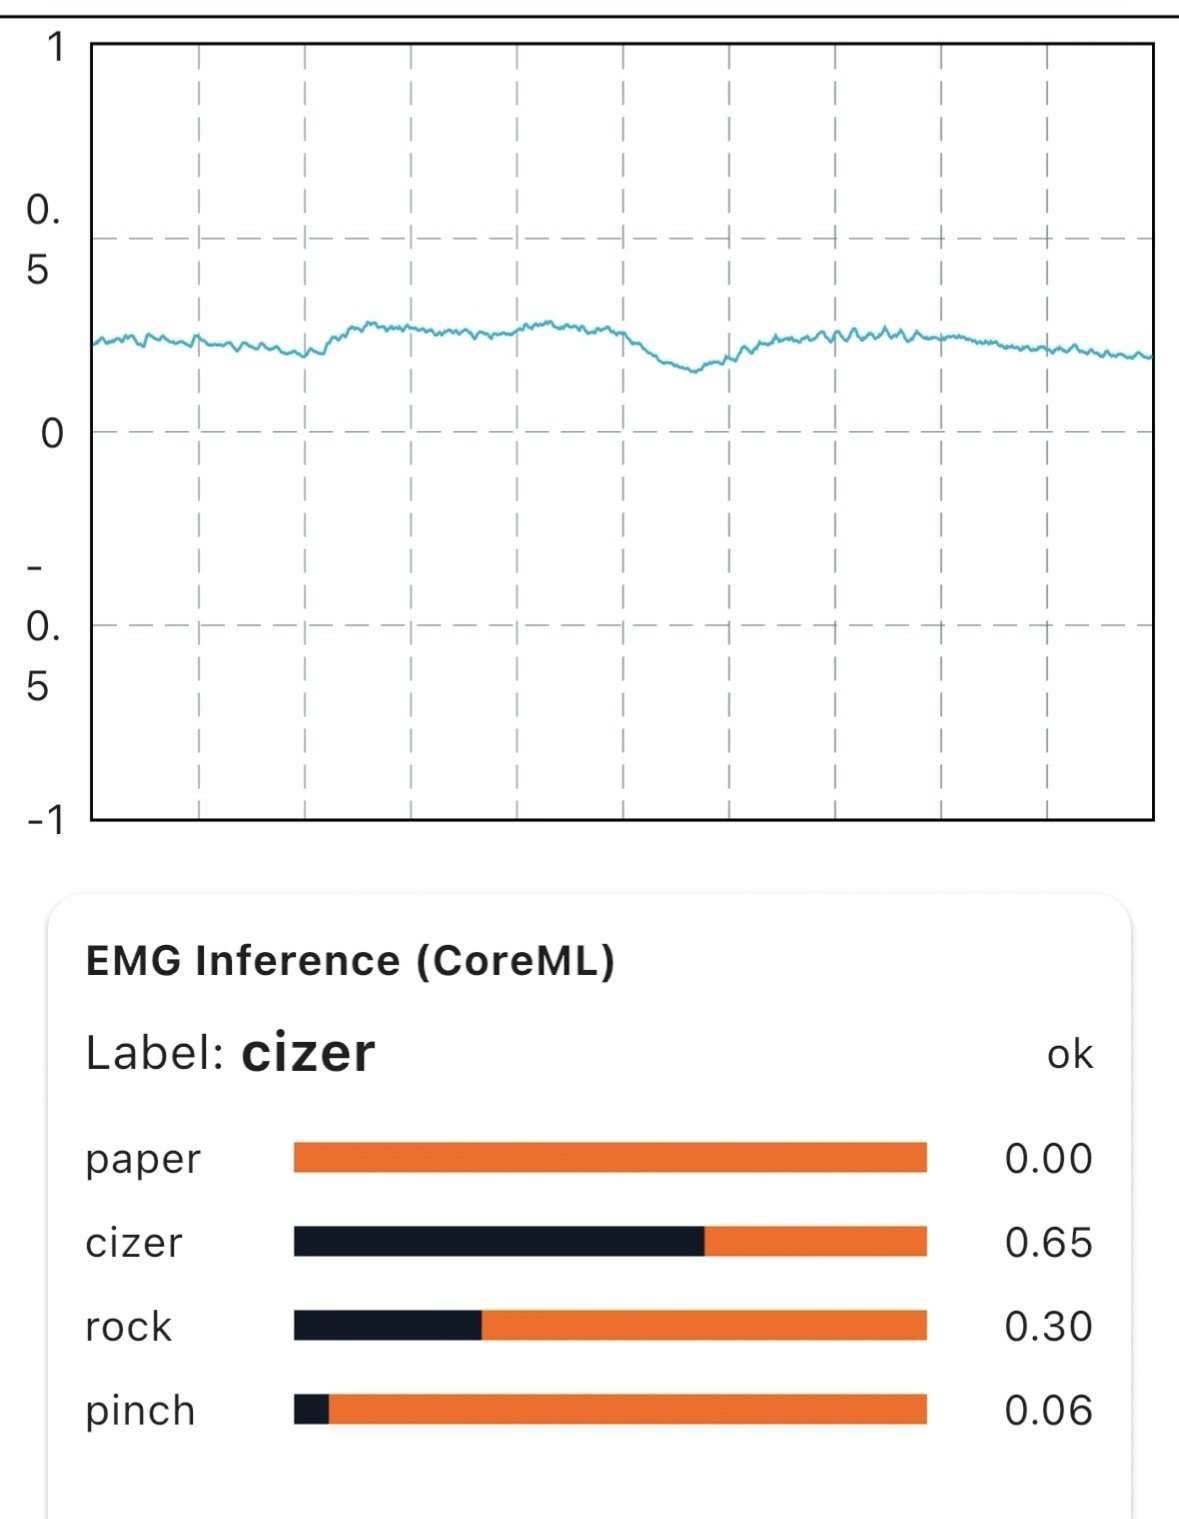
\includegraphics[width=0.35\linewidth]{src/realtiime_inference_screen.jpg}
    \caption{リアルタイム推論画面（波形表示と確率分布）}
    \label{fig:realtime-inference}
\end{figure}

\subsubsection{推論結果の可視化}
図\ref{fig:realtime-inference}に示すように,
画面上部には正規化されたsEMG波形をリアルタイムで表示し,
下部には現在の推論結果を表示する.
各ジェスチャ（paper, cizer, rock, pinch）の確率をプログレスバーで視覚化し,
最も確率の高いラベルを強調表示する.

\subsubsection{精度測定機能}
定量的な性能評価のため,ラベルごとの認識精度を測定する機能を実装した（図\ref{fig:accuracy-measurement}）.
ユーザーが特定のジェスチャを実行しながらラベルボタンを押下すると,
3秒間の推論結果を集計し,正解率を算出する.

測定ロジックは以下の通り：
\begin{itemize}
\item 測定中フラグ（\texttt{\_measuring}）をtrueに設定
\item 測定対象ラベル（\texttt{\_measuringLabel}）を記録
\item 3秒間,各推論結果の\texttt{labelIndex}が測定対象と一致するか判定
\item 正解数/総推論回数から精度（\%）を算出
\item 結果をプログレスバーで可視化（緑：80\%以上,オレンジ：60-80\%,赤：60\%未満）
\end{itemize}

この機能により,On-device学習前後の精度変化や,
ユーザー固有パターンへの適応度を定量的に評価できる.
\begin{figure}[htbp]
\centering
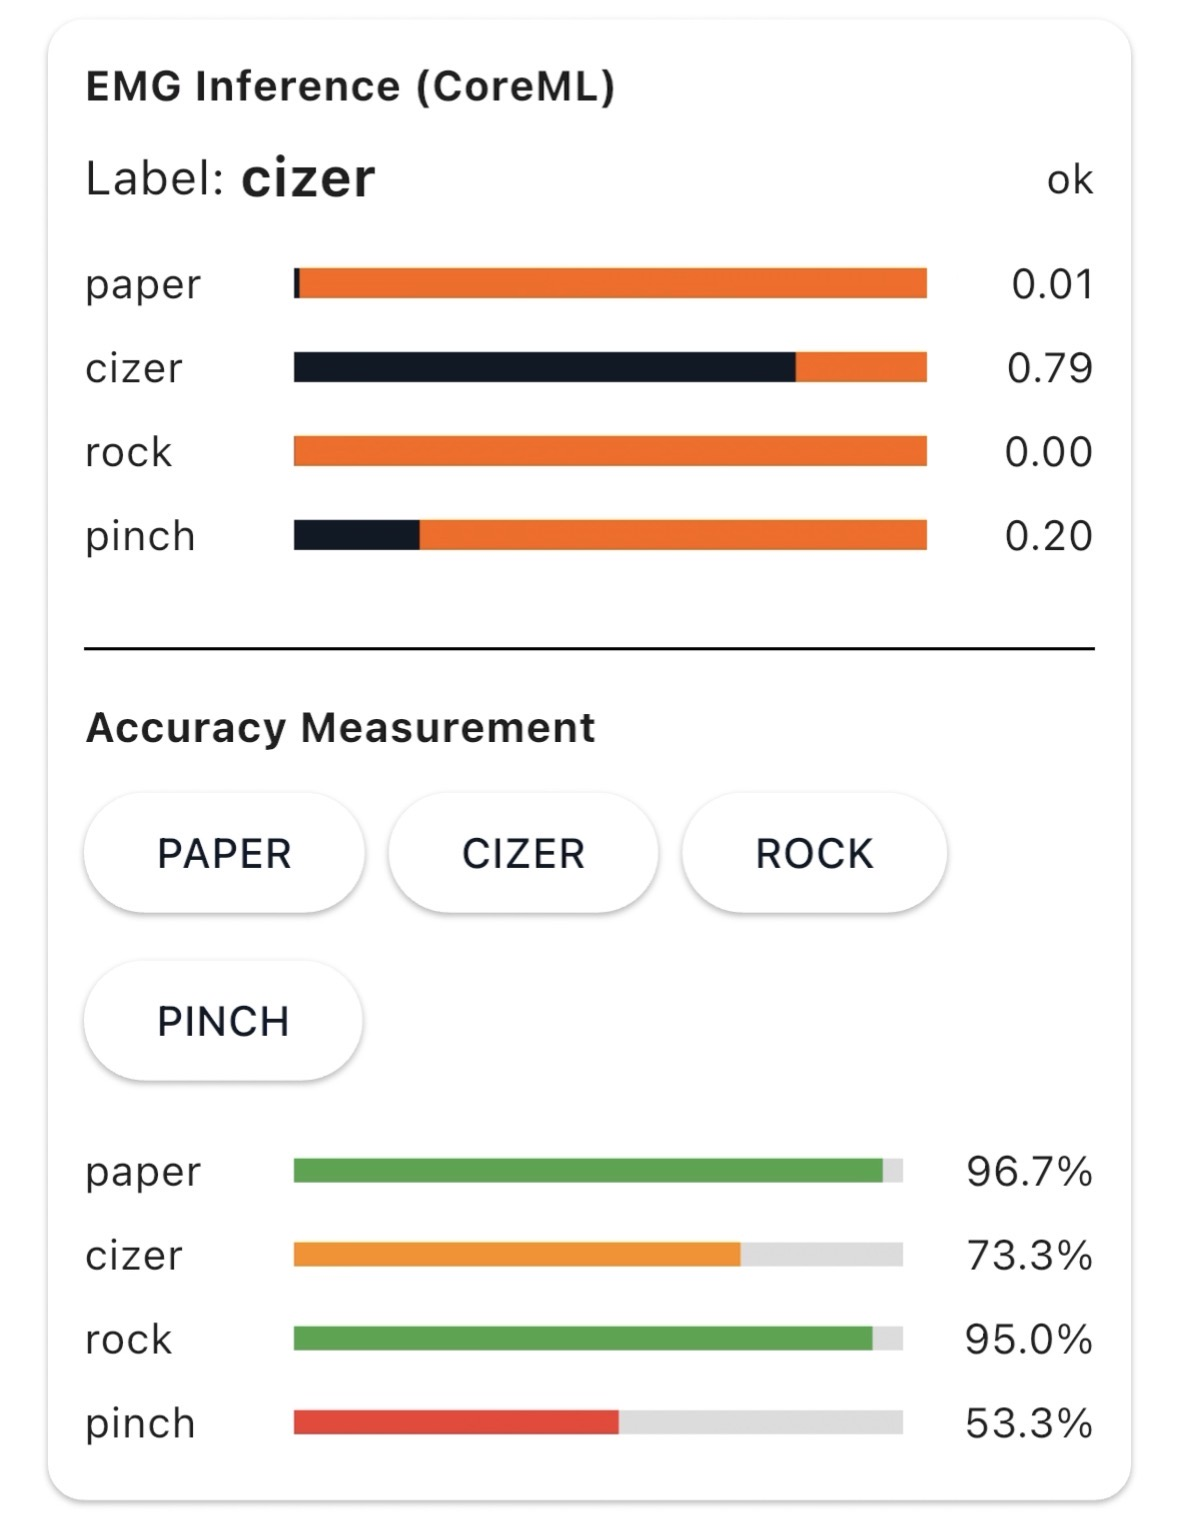
\includegraphics[width=0.35\linewidth]{src/inference_analize_screen.jpg}
\caption{精度測定画面（ラベルごとの認識精度）}
\label{fig:accuracy-measurement}
\end{figure}

\subsection{データセット記録とOn-device学習}
On-device学習によるユーザー適応を実現するため,
ラベル付きデータセットの収集・保存・学習機能を実装した.
この機能は\texttt{EmgDatasetRecorder}（\ref{subsubsec:dataset-recorder}）を中心に,
複数のServiceを統合して動作する.

\subsubsection{データセット記録フロー}
ユーザーは記録したいジェスチャのボタンを押下することで,
そのジェスチャに対応するラベル付きデータを自動収集できる.



ボタン押下中,以下の処理が自動実行される：
\begin{enumerate}
\item BleServiceからリアルタイムでパケット受信
\item EmgWindowBufferで150ms/50msホップのウィンドウ切り出し
\item EmgFeatureExtractorで10次元特徴量抽出
\item \texttt{\{features: [10次元], classLabel: "label", timestamp: "ISO8601"\}}形式でメモリに蓄積
\item 画面上部に蓄積行数（rows in memory）を表示
\end{enumerate}

\begin{figure}[htbp]
    \centering
    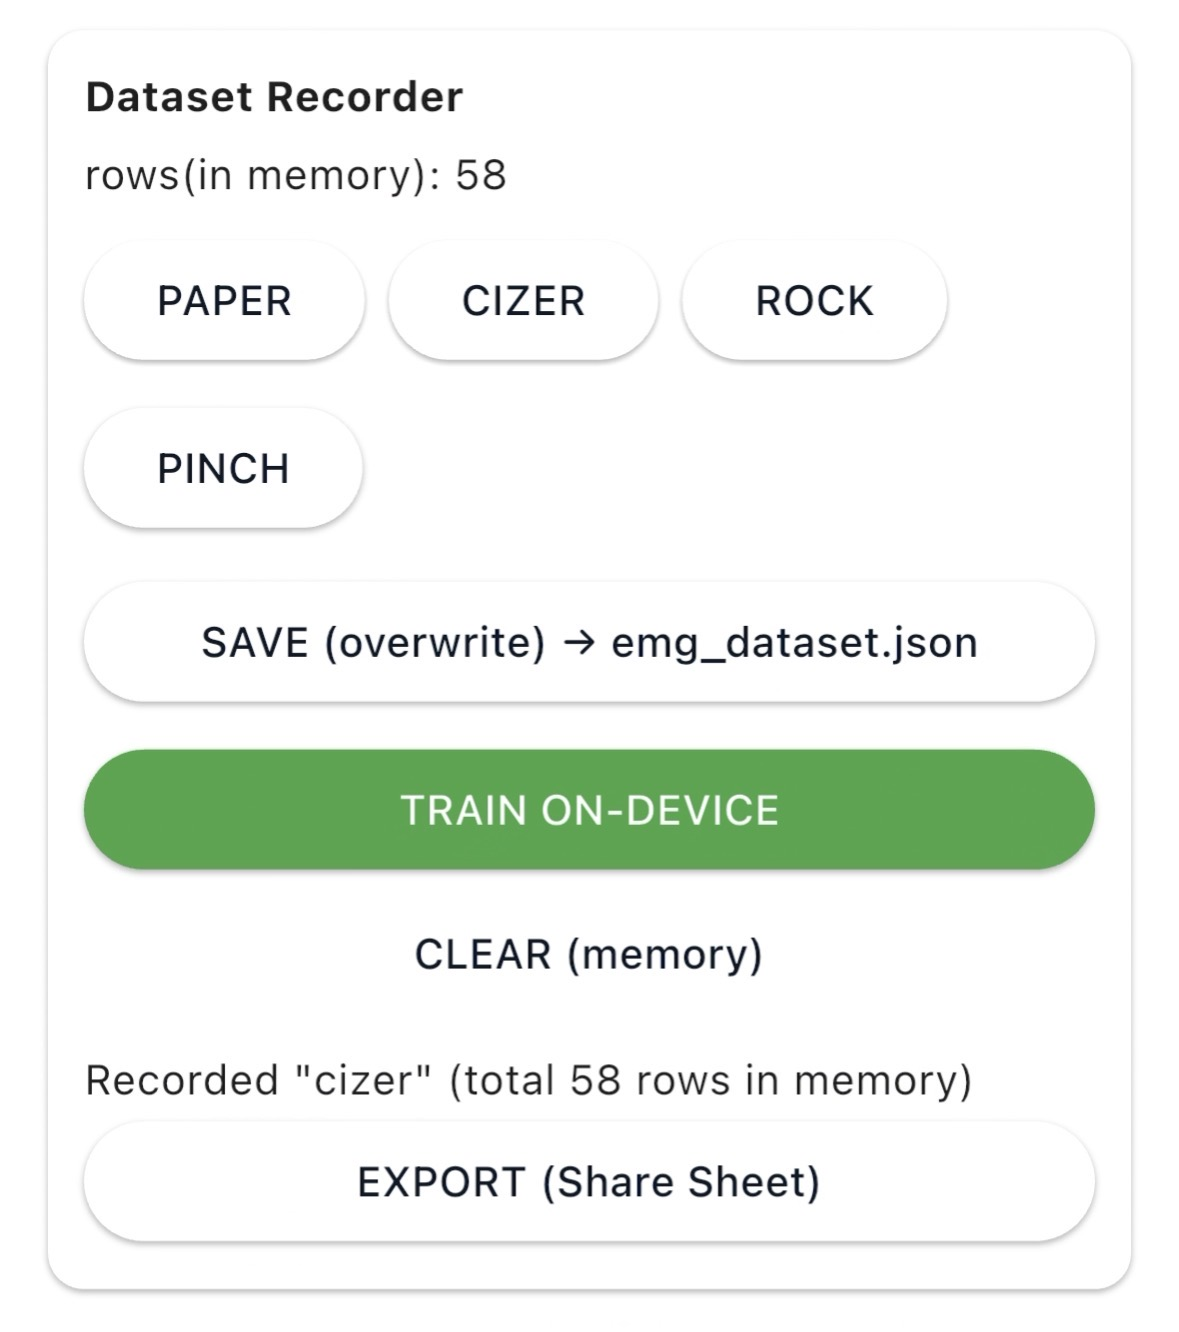
\includegraphics[width=0.35\linewidth]{src/dateset_recorder_screen.jpg}
    \caption{データセット記録画面（ラベル選択と保存・学習）}
    \label{fig:dataset-recorder}
\end{figure}

この方式により,ユーザーは複数のジェスチャを順次記録し,
1つのセッション内で多クラスのデータセットを構築できる.



\subsubsection{データの保存とエクスポート}
収集したデータセットは,以下の2つの用途で利用される：

\paragraph{1. JSON保存（ローカルストレージ）}
\texttt{SAVE (overwrite) → emg\_dataset.json}ボタンにより,
メモリ上のデータセットを\texttt{getApplicationDocumentsDirectory()}配下にJSON形式で保存する.
ファイルフォーマットは以下の通り:
\begin{verbatim}
[
  {"features": [f0,...,f9], "classLabel": "paper", "ts": "..."},
  {"features": [f0,...,f9], "classLabel": "cizer", "ts": "..."},
  ...
]
\end{verbatim}

\paragraph{2. エクスポート（外部解析用）}
\texttt{EXPORT (Share Sheet)}ボタンにより,
保存したJSONファイルをiOSのShare Sheet経由でエクスポートできる.
これにより,以下の用途に利用可能となる：
\begin{itemize}
\item Pythonスクリプトによるオフライン解析
\item 事前学習用データセットとしての活用
\item 論文執筆時の実験データとしての保管
\end{itemize}

\subsubsection{On-device学習の実行}
\texttt{TRAIN ON-DEVICE}ボタンにより,
収集したデータセットを用いてCore MLモデルの重みを更新する.
内部では以下の処理が実行される：
\begin{enumerate}
\item メモリ上のデータセットを\texttt{LabeledEmgSample}のリストに変換
\item EmgMlService（\ref{subsubsec:ml-service}）の\texttt{train()}メソッド呼び出し
\item Method Channel経由でiOS Native層に送信
\item Core MLの\texttt{MLUpdateTask}でNeural Engine上で学習実行
\item 学習後の重みを永続化（次回起動時に自動ロード）
\end{enumerate}

学習完了後,前述の精度測定機能（\ref{fig:accuracy-measurement}）により,
適応前後の性能変化を定量的に確認できる.

\subsubsection{メモリクリア}
\texttt{CLEAR (memory)}ボタンにより,
メモリ上のデータセットを消去し,新しいセッションを開始できる.
これにより,異なる条件でのデータ収集を繰り返し実行可能となる.




